
Nel capitolo precedente è stata descritta l'architettura generale del progetto, inclusa l'infrastruttura su cui saranno distribuiti i moduli Wasm. In questo capitolo verranno approfonditi i dettagli dello sviluppo del framework protagonista di questo elaborato di tesi, già presentato ad alto livello nella Sez. \ref{sec:framework_structure}.\\  
Il framework, denominato PELATO, è un acronimo di \textbf{Progettazione ed Esecuzione di Lifecycle Automatizzati e Tecnologie d'Orchestrazione per moduli WebAssembly} ed ha lo scopo di fornire gli strumenti per poter generare, buildare e deployare un componente Wasm partendo dalla semplice definizione di una funzione.\\

\section{Tecnologie utilizzate}

In questa sezione verranno elencate e spiegate le tecnologie utilizzate per lo sviluppo di questa soluzione. Per quanto riguarda WebAssembly e gli argomenti correlati sono già stati ampiamente descritti nella sezione [\ref{sec:webassembly}], quindi ci concentreremo principalmente sui linguaggi e i tool utilizzati dal framework PELATO, iniziando dal linguaggio in cui è stato programmato.

\subsection{Python}

Python è un linguaggio di programmazione ad alto livello, interpretato e orientato agli oggetti, ideato da Guido van Rossum e rilasciato per la prima volta nel 1991. Nel corso degli anni, Python si è affermato come uno degli strumenti più diffusi e versatili nel panorama della programmazione, grazie a una combinazione di semplicità, leggibilità e potenza espressiva.\\
Una delle qualità distintive di Python è la sua sintassi chiara e intuitiva, che facilita sia l'apprendimento per i principianti che la manutenzione del codice in progetti di grandi dimensioni. La tipizzazione dinamica permette di scrivere codice in maniera rapida, senza la necessità di dichiarazioni esplicite dei tipi, rendendo lo sviluppo più fluido ed efficiente.\\
Python vanta un ampio ecosistema di librerie e framework, che lo rende adatto a molteplici applicazioni, dalla scienza dei dati allo sviluppo web, accelerando la realizzazione di progetti complessi. Supporta vari paradigmi (procedurale, orientato agli oggetti, funzionale) e gestisce automaticamente la memoria tramite il garbage collector, riducendo il rischio di errori legati alla gestione delle risorse. Inoltre, la sua elevata portabilità su piattaforme diverse (Windows, macOS, Linux) lo rende ideale sia per la prototipazione rapida che per soluzioni enterprise.

\subsubsection{Motivi dell'utilizzo}
La scelta di impiegare questo linguaggio per sviluppare il framework è stata motivata principalmente dalla vasta gamma di librerie disponibili, che agevolano l'uso di strumenti come Jinja e facilitano l'integrazione con sistemi quali Docker, essenziali per la generazione e compilazione del codice.\\
È noto che Python, pur offrendo un ecosistema ricco e una sintassi intuitiva, può presentare limitazioni in termini di performance, soprattutto per operazioni CPU-intensive. Questo è in gran parte dovuto al Global Interpreter Lock (GIL), che impedisce l'effettivo sfruttamento del multi-threading in scenari di calcolo parallelo. Questi problemi sono stati risolti spostando il carico computazionale ed il parallelismo su strumenti esterni come Docker (la metodologia verrà spiegata in seguito).

\subsubsection{Jinja}
Jinja è un motore di template per Python che consente di generare contenuti dinamici combinando testo statico e logica di programmazione. La sua sintassi semplice e flessibile lo rende adatto a numerosi contesti applicativi, dalla generazione di pagine web fino all'automazione di configurazioni.\\
Oltre al suo utilizzo in framework web come Flask e in strumenti di automazione come Ansible, Jinja può essere impiegato anche nella generazione di file di configurazione per orchestratori di container come Helm. Ad esempio, all'interno degli Helm Chars, è possibile usare Jinja per parametrizzare i valori nei file di configurazione di Kubernetes:

\begin{lstlisting}[language=yaml]
apiVersion: v1
kind: ConfigMap
metadata:
  name: {{ .Values.configMapName }}
data:
  key: {{ .Values.configKey }}
\end{lstlisting}

In questo caso, i valori racchiusi tra le doppie parentesi graffe vengono sostituiti con i corrispondenti parametri definiti nel file \texttt{values.yaml}, permettendo una configurazione dinamica e facilmente riutilizzabile.\\
L'approccio utilizzato nel framework è lo stesso: infatti Jinja viene utilizzato per generare il codice sostituendo le variabili contenute nei templates con quelle del file \texttt{workflow.yaml}.

\subsubsection{Integrazione con Docker}

La libreria \texttt{docker-py} permette di interagire con l'API di Docker direttamente da applicazioni Python, facilitando la gestione e l'automazione dei container. Questa libreria consente di eseguire operazioni come la creazione, l'avvio e l'eliminazione di container, nonché la gestione di immagini e volumi.\\
Ad esempio, è possibile creare ed eseguire un container tramite poche righe di codice:

\begin{lstlisting}[language=python]
import docker

client = docker.from_env()
container = client.containers.run("nginx", detach=True, ports={'80/tcp': 8080})
print(f"Container avviato con ID: {container.id}")
\end{lstlisting}

L'integrazione con Docker semplifica l'automazione di processi di deployment e testing, rendendo Python uno strumento efficace per lo sviluppo e la gestione di applicazioni containerizzate. Inoltre permette di delegare l'esecuzione di task onerose ad ambienti ottimizzati e parallelizzare l'operazione (approccio utilizzato in fase di Build e Deployment).

\subsection{Golang}

Golang, comunemente noto come Go, è un linguaggio di programmazione open source sviluppato da Google nel 2007 e rilasciato pubblicamente nel 2009. Il linguaggio è stato progettato con l'obiettivo di combinare l'efficienza e la sicurezza della programmazione statica con la semplicità e la produttività tipiche dei linguaggi dinamici.\\
Grazie alla sua sintassi concisa e alla gestione efficiente della concorrenza, Go è diventato rapidamente uno strumento di riferimento per la creazione di applicazioni scalabili e ad alte prestazioni.\\
Go si distingue per la sua tipizzazione statica, il garbage collection integrato e il sistema di concorrenza basato sulle goroutine, che consente di eseguire migliaia di operazioni concorrenti con un overhead minimo. Il linguaggio supporta la programmazione orientata agli oggetti attraverso l'uso di interfacce e strutture (structs), pur mantenendo una filosofia minimalista e pragmatica. Inoltre, la standard library di Go fornisce un ricco set di funzionalità, tra cui strumenti per la gestione della rete, il parsing di file e la sicurezza crittografica.\\

\subsubsection{Integrazione con WebAssembly}
Con l'avvento delle applicazioni web moderne e della necessità di eseguire codice ad alte prestazioni nel browser, Go ha introdotto il supporto per WebAssembly (Wasm) a partire dalla versione 1.11. L'integrazione avviene attraverso la compilazione del codice sorgente in un file binario Wasm utilizzando il comando:

\begin{lstlisting}[language=bash]
go build -o main.wasm -tags=wasm main.go
\end{lstlisting}

L'integrazione con Wasm è supportata anche da TinyGo, un compilatore alternativo progettato per ambienti con risorse limitate come i microcontrollori. Supporta la compilazione di programmi Go sia per l'esecuzione nei browser (WASM) sia su server e dispositivi edge tramite WASI.\\
Questa integrazione consente agli sviluppatori di scrivere codice Go idiomatico e compilarlo in moduli WebAssembly che possono interagire direttamente con l'ambiente host attraverso le interfacce fornite da WASI. Inoltre supporta l'ultima specifica di WASI (P vreview 0.2, descritta nella sezione [\ref{sec:wasi}]) consentendo di compilare dei componenti conformi con la specifica OCI.\\
Date queste caratteristiche Go è il linguaggio che è stato scelto per lo modellare i template e per l'implementazione delle task del modello FaaS.

\section{Struttura del framework}

Il framework è sviluppato secondo un'architettura che adotta il pattern di progettazione \texttt{Facade} che fornisce un'interfaccia semplificata e unificata per un accedere alle varie funzionalità. In pratica, una classe Facade funge da punto di accesso centrale, nascondendo la complessità interna e offrendo metodi di alto livello per interagire con il sistema.\\
La classe \texttt{Pelato} viene utilizzata come punto di accesso per la CLI (command line interface), memorizza le configurazioni iniziali e si occupa di salvare le metriche. Inoltre è responsabile dell'esecuzione della logica di business implementata nei tre package:
\begin{itemize}
    \item \texttt{code\_generator}
    \item \texttt{wasm\_builder}
    \item \texttt{component\_deploy}
\end{itemize}

La configurazione iniziale della classe avviene tramite variabili d'ambiente (che possono essere caricate dal framework tramite un file \texttt{.env} locale, verranno dati più dettagli in seguito); ciò consente una facile implementazione del framework come applicazione containerizzata, nel caso si volesse ``trasformare" in un servizio gestito in Cloud.\\
Questo pattern di progettazione aumenta la modularità dei componenti facilitando eventuali estensioni, come quella mostrata nella figura [\ref{fig:pelato_architecture}], dove si fa l'esempio di un API Server affiancato alla CLI).\\

\FloatBarrier
\begin{figure}[h]
    \centering
    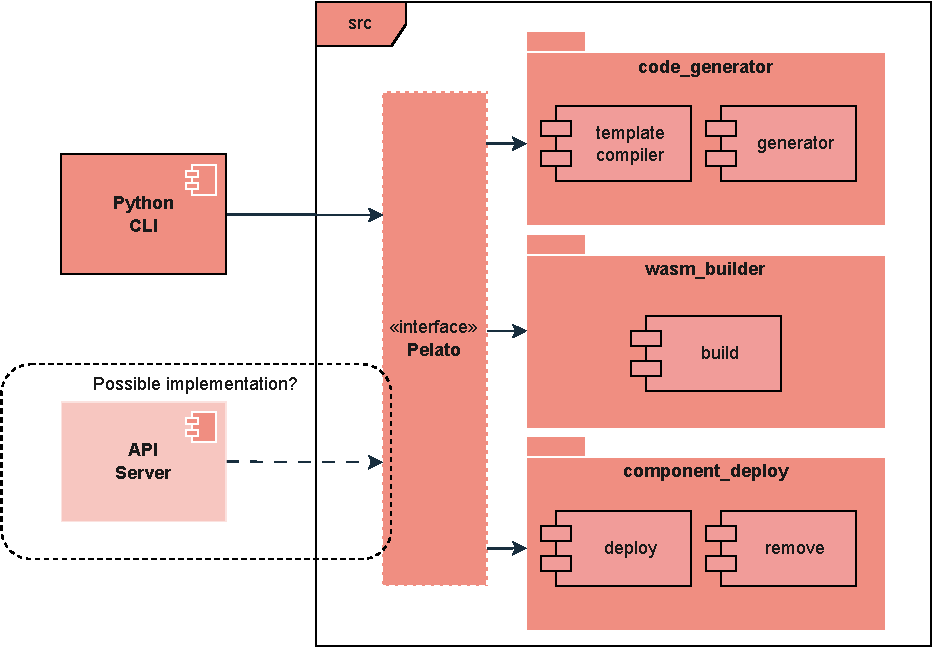
\includegraphics[width=0.8\textwidth]{img/schemi/schemi-implementazione-struttura.drawio.pdf}
    \caption{Architettura framework PELATO}
    \label{fig:pelato_architecture}
\end{figure}
\FloatBarrier

\subsection{Python CLI}

Come già anticipato in precedenza l'interfacciamento fra utente e framework è realizzata tramite una CLI, cioè un'interfaccia a riga di comando in grado di ricevere istruzioni e configurazioni.\\
Per invocare la CLI è sufficiente lanciare il comando \lstinline{python3 pelato.py}, che restituirà come output le varie opzioni e gli argomenti necessari:\\
\begin{lstlisting}[caption={Output Pelato CLI}, captionpos=b, label={code:pelato_cli}]
    usage: pelato.py [-h] {gen,build,deploy,remove,brush} ...

    Generate, build and deploy WASM components written in go
    
                        Command list
    gen                 Generate Go code
    build               Build WASM component
    deploy              Deploy WASM components
    remove              Remove deployed WASM components
    brush               Starts the pipeline: gen -> build -> deploy

    options:
      -h, --help            show this help message and exit
\end{lstlisting}

Ogni operazione della cli deve essere invocata specificando la directory progetto, cioè quella in cui si trovano il file \texttt{workflow.yaml} e la cartella contenente le task, per esempio

\begin{lstlisting}[language=bash, caption={Invocazione Pelato CLI}, captionpos=b, label={code:pelato_cli_brush}]
    $ python3 pelato.py brush project/
\end{lstlisting}

Oltre alle tre operazioni richieste, cioè gen, build e deploy, la CLI permette di eseguire anche:
\begin{itemize}
    \item \textbf{brush} -- lancia l'intera pipeline di gen, build e deploy
    \item \textbf{remove} -- utile per rimuovere le applicazioni deployate tramite la CLI (devono essere ancora presenti i files utilizzati per la fase di deploy)
\end{itemize}

\subsection{Code generator}

Andiamo ora a descrivere il dettaglio il meccanismo di generazione del codice. Il package è composto dai seguenti file:

\dirtree{%
.1 code\_generator/.
.1 generator.py.
.1 template\_compiler.py.
.1 templates/.
.2 processor\_nats/.
.2 producer\_nats/.
}

Analizziamo ora nel dettaglio il processo di generazione del codice, partendo dalla fase di analisi del progetto fornito dall'utente. La prima operazione viene effettuata da \texttt{generator.py}, di cui riportiamo un estratto contenente il codice più rilevante e che corrisponde allo schema riportato in fasi di analisi dell'architettura [\ref{fig:code_gen_pipeline}].
\begin{lstlisting}[language=python, caption={Generazione del codice}, captionpos=b, label={code:code_gen}]
    def generate(project_dir, registry_url, metrics, metrics_enabled):
        ...
        # Parsing del file workflow.yaml
        config = __parse_yaml(f"{project_dir}/workflow.yaml")
        
        # Pulizia della cartella di output
        __remove_dir_if_exists(output_dir)
        os.makedirs(output_dir, exist_ok=True)
        
        # Per ogni task all'interno del file workflow
        for task in config['tasks']:
            ...
            # Compilazione dei template
            template_compiler.handle_task(task, output_dir)

            # Copia del file task all'interno della cartella di output
            shutil.copy2(f"{project_dir}/tasks/{task['code']}", f"{output_dir}/{task['component_name']}/{task['code']}")
                
        if metrics_enabled:
            gen_metrics['gen_time'] = '%.3f'%(end_time - start_time)
            metrics['code_gen'] = gen_metrics
\end{lstlisting}

Come si può notare dal codice la funzione si occupa di parsare il file workflow e controllarne la validità e preparare la cartella di output. La generazione vera e propria del codice viene affidata a \texttt{template\_compiler} tramite la funzione \texttt{handle\_task}, la quale seleziona il template corretto in base a quello riportato nella configurazione, lo copia nella cartella di output e lo compila utilizzando Jinja.\\
Di seguito viene riportato un esempio di file (in questo caso una porzione di \texttt{wadm.yaml}) prima e dopo la compilazione del template tramite Jinja.\\

\noindent\begin{minipage}{.46\textwidth}
\begin{lstlisting}[caption=Template wadm.yaml, language=yaml, basicstyle=\scriptsize, frame=single]
spec:
  components:
    - name: {{ component_name }}
      type: component
      properties:
        image: "{{ registry_url }}/{{ component_name }}:{{ version }}"
      traits:
        - type: link
          properties:
            target: nats-processor
            namespace: wasmcloud
            package: messaging
            interfaces: [consumer]
        - type: spreadscaler
          properties:
            instances: 1
            spread:
            
            
            - name: {{ target }}
              weight: {{ weight }}
              requirements:
                host-type: {{ target }}
            
\end{lstlisting}
\end{minipage}
\hfill
$\rightarrow$
\hfill
\begin{minipage}{.46\textwidth}
\begin{lstlisting}[caption=wadm.yaml compilato con Jinja, language=yaml, basicstyle=\scriptsize, frame=single]
spec:
  components:
    - name: data_double_test1
      type: component
      properties:
        image: "gitea.rebus.ninja/lore/data_double_test1:1.0.0"
      traits:
        - type: link
          properties:
            target: nats-processor
            namespace: wasmcloud
            package: messaging
            interfaces: [consumer]
        - type: spreadscaler
          properties:
            instances: 1
            spread:
            - name: cloud
              weight: 100
              requirements:
                host-type: cloud
\end{lstlisting}
\end{minipage}

A questo punto viene copiato il file specificato sulla configurazione dalla cartella \texttt{task/} del progetto alla cartella di output. La funzione viene automaticamente agganciata all'handler specifico del template, la specifica esatta della costruzione del file task verrà approfondita in seguito.\\
L'intero processo di generazione può essere rappresentato dal seguente schema [\ref{fig:code_gen_impl}]:

\FloatBarrier
\begin{figure}[h]
    \centering
    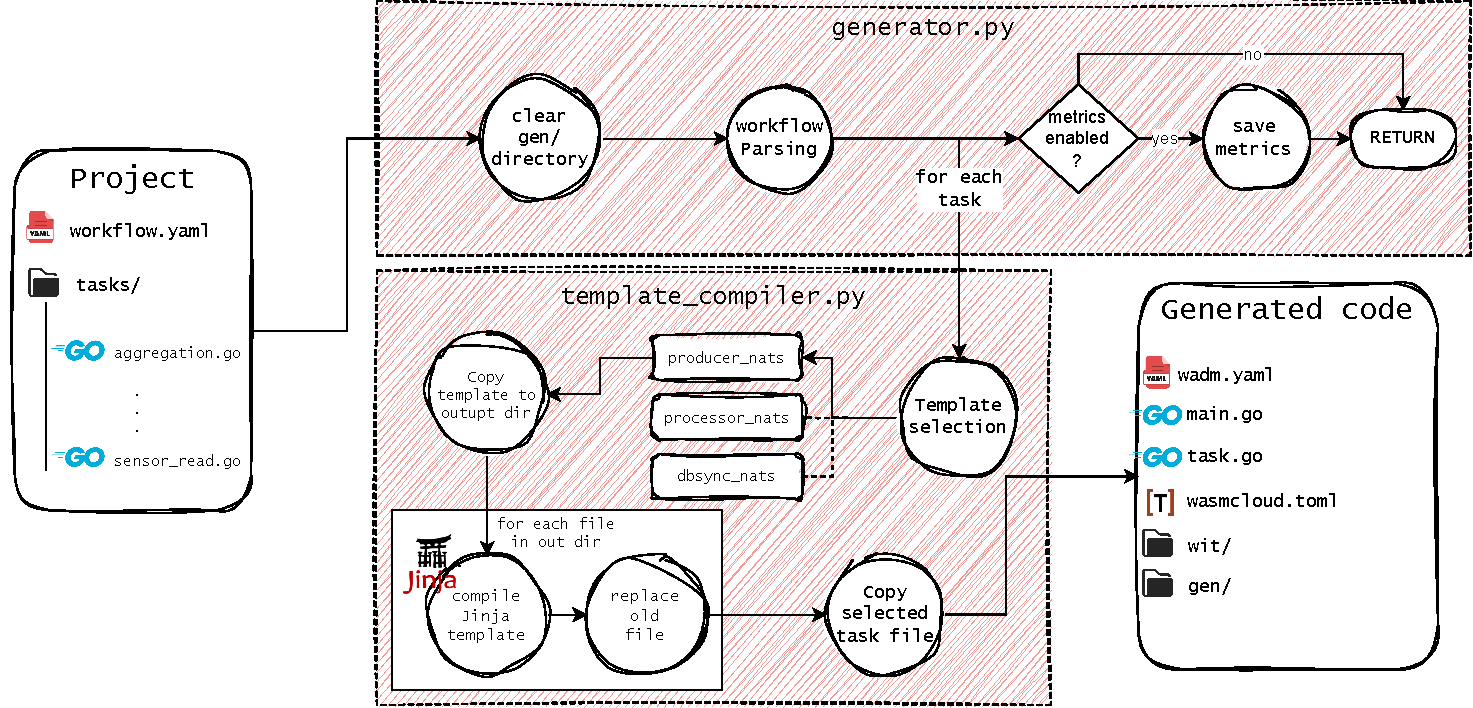
\includegraphics[width=\textwidth]{img/schemi/schemi-implementazione-gen.drawio.pdf}
    \caption{Processo generazione del codice}
    \label{fig:code_gen_impl}
\end{figure}
\FloatBarrier

\subsection{Wasm builder}

Se la fase di generazione è avvenuta con successo, all'interno del progetto dovrebbe essere presente una cartella chiamata \texttt{gen}, contenente diverse sotto-cartelle con il codice necessario per compilare i moduli Wasm.

\texttt{project/}
\dirtree{%
.1 workflow.yaml.
.1 tasks/.
.1 gen/.
.2 example\_component1.
.2 example\_component2.
}

A questo punto può essere invocato il componente \texttt{build}, che sostanzialmente esegue le seguenti operazioni:
\begin{enumerate}
    \item istanzia il client Docker utilizzando l'apposito SDK\footnote{\url{https://pypi.org/project/docker/}}
    \item controlla se l'immagine \texttt{wash-build-image:latest} è presente. Se non lo è procede a buildarla utilizzando il dockerfile configurato
    \item per ogni cartella presente dentro \texttt{gen} istanzia un container con \texttt{wash-build-image} come immagine e monta la cartella all'interno del container
    \item attende la terminazione dei container
\end{enumerate}

Si può notare come in questo caso le operazioni svolte dal framework siano limitate: la logica di build del componente e la pubblicazione dell'artifact OCI sono infatti delegate alle istanze in esecuzione su Docker.
    
\subsubsection{Wash build image}

Approfondiamo ora il meccanismo utilizzato per buildare i componenti Wasm, iniziando dal Dockerfile che descrive l'immagine di base utilizzata:

\begin{lstlisting}[language=Dockerfile, caption={wash-build-image Dockerfile}, captionpos=b, label={code:wash_buil_image_dockerfile}, basicstyle=\ttfamily\small]
FROM ubuntu:24.04 AS wash-build-image

# Install dependencies and tools
RUN apt-get update && apt-get install -y curl wget tar ...

# ----------------- Install WasmCloud -----------------
RUN curl -s "https://packagecloud.io/install/repositories/wasmcloud/core/script.deb.sh" | bash && \
    apt-get install -y wash

# ----------------- Install Go 1.23 -----------------    
RUN wget https://go.dev/dl/go1.23.4.linux-amd64.tar.gz && \
    tar -C /usr/local -xzf go1.23.4.linux-amd64.tar.gz && \
    rm go1.23.4.linux-amd64.tar.gz

# Set Go environment variables
ENV PATH="/usr/local/go/bin:${PATH}"
ENV GOPATH="/go"
ENV GOROOT="/usr/local/go"

# ----------------- Install TinyGo 0.34.0 -----------------
RUN wget https://github.com/tinygo-org/tinygo/releases/download/v0.34.0/tinygo_0.34.0_amd64.deb && \
    dpkg -i tinygo_0.34.0_amd64.deb && \
    rm tinygo_0.34.0_amd64.deb

# ----------------- Install Rust -----------------
# Install Rust
RUN curl https://sh.rustup.rs -sSf | sh -s -- -y && \
    . "$HOME/.cargo/env" && \
    cargo install --locked wasm-tools

# Set Rust environment variables
ENV PATH="/root/.cargo/bin:${PATH}"

# Verify installations
RUN go version && tinygo version && cargo --version && wash --version && wasm-tools --version

# ----------------- Build the WasmCloud module -----------------
FROM wash-build-image

RUN mkdir /app
WORKDIR /app

# Install go dependencies, build the wasm module, push it to the registry
CMD ["sh", "-c", "go env -w GOFLAGS=-buildvcs=false && go mod download && go mod verify && wash build && wash push $REGISTRY build/*.wasm && chown -R ${HOST_UID}:${HOST_GID} ."]
\end{lstlisting}

Il Dockerfile è strutturato in due fasi, nella prima vengono installate le dipendenze di Go, TinyGo, Rust e la shell di wasmCloud. Nella seconda fase viene predisposta l'immagine per la compilazione dei moduli Wasm; nell'istruzzione CMD infatti troviamo:
\begin{itemize}
    \item istruzioni per risolvere le dipendenze di go ed installarle nel progetto
    \item comando \texttt{wash build} che esegue la compilazione del progetto e genera il componente Wasm all'interno della cartella \texttt{gen}
    \item comando \texttt{wash push} che carica il file Wasm sul registry configurato come OCI artifact
    \item istruzione per impostare i corretti permessi sui file generati
\end{itemize}

Questo approccio consente di utilizzare una sola immagine per tutte le operazioni di build: le configurazioni dinamiche avvengono tramite variabili d'ambiente e i file da buildare vengono montati come volume al posto della cartella \texttt{/app}, come possiamo notare dal seguente estratto di codice del componente \texttt{build}:

\begin{lstlisting}[language=python, caption={Build componente Wasm con Docker}, captionpos=b, label={code:build}]
def __build_wasm(task_dir, client, reg_user, reg_pass, detached, wait_list):
    oci_url = wadm['spec']['components'][0]['properties']['image']
    name = wadm['spec']['components'][0]['name'] + '-build'
    ...
    # Build componente Wasm
    print(f" - Building WASM module {oci_url}")
    container = client.containers.run(
        "wash-build-image:latest",
        environment=[f'REGISTRY={oci_url}',
                     f'WASH_REG_USER={reg_user}',
                     f'WASH_REG_PASSWORD={reg_pass}',
                     f'HOST_UID={uid}',
                     f'HOST_GID={gid}'],
        volumes={os.path.abspath(task_dir): {'bind': '/app', 'mode': 'rw'}},
        remove = True,
        detach = True,
        name = name
    )
    
    # Build sequenziale o parallela
    if detached == 'False':
        container.wait()
    else:
        wait_list.append(name)
\end{lstlisting}

Il processo di build può essere eseguito in modalità sequenziale o parallela, a seconda della configurazione delle variabili d'ambiente. Questo comportamento è gestito tramite la flag \texttt{detach}, che permette di avviare i container in modo asincrono. In questa modalità, viene utilizzata una waiting list per istanziare tutti i container in parallelo e attendere il completamento dell'operazione di build.\\
L'intero processo di build viene mostrato nella seguente immagine [\ref{fig:impl_build}]:

\FloatBarrier
\begin{figure}[h]
    \centering
    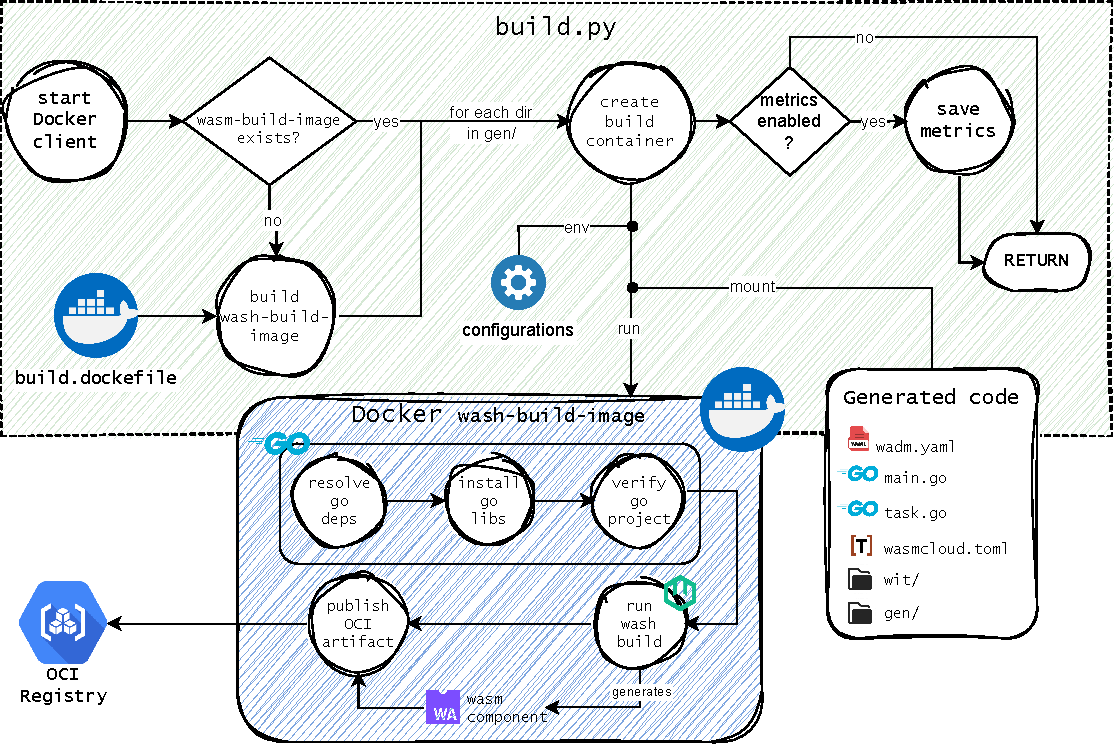
\includegraphics[width=\textwidth]{img/schemi/schemi-implementazione-build.drawio.pdf}
    \caption{Processo di Build componente Wasm}
    \label{fig:impl_build}
\end{figure}
\FloatBarrier

\subsection{Component deploy}

La fase di deployment è strutturata in modo molto simile a quella di build, infatti le operazione svolte dal componente deploy sono:

\begin{enumerate}
    \item istanziamento del client Docker
    \item controllo dell'immagine \texttt{wash-deploy-image:latest}, se non è presente procede a buildarla utilizzando il dockerfile configurato
    \item per ogni cartella presente dentro \texttt{gen} istanzia un container con \texttt{wash-deploy-image} come immagine e monta la cartella all'interno del container
    \item attende la terminazione dei container
\end{enumerate}

 Il Dockerfile utilizzato per buildare l'immagine \texttt{wash-deploy-image} è più semplice, in quanto deve solamente installare la wasmCloud shell e le sue dipendenze:
 
\begin{lstlisting}[language=Dockerfile, caption={wash-build-image Dockerfile}, captionpos=b, label={code:wash_buil_image_dockerfile}, basicstyle=\ttfamily\small]
FROM ubuntu:24.04 AS wash-deploy-image

# Install dependencies and tools
RUN apt-get update && apt-get install -y curl wget tar ...

# ----------------- Install WasmCloud -----------------
RUN curl -s "https://packagecloud.io/install/repositories/wasmcloud/core/script.deb.sh" | bash && \
    apt-get install -y wash

# ----------------- Deploy the WasmCloud module -----------------
FROM wash-deploy-image

RUN mkdir /app
WORKDIR /app

# Deploy the WasmCloud module
CMD ["sh", "-c", "wash app deploy wadm.yaml"]
\end{lstlisting}

Il comando riporato nell'istruzione CMD in questo caso è \texttt{wash app deploy wadm.yaml}, che utilizza il file wadm.yaml per creare un applicazione sul cluster wasmCloud specificato.\\
L'approccio utilizzato per eseguire i processi di deployment è analogo a quello della fase Build, la differenza sta nelle variabili d'ambiente necessarie all'operazione: in questo caso sarà necessario fornire hostname e porta di un server NATS collegato al cluster wasmCloud. Di seguito viene riportata la porzione di codice che si occupa di eseguire il container.\\

\begin{lstlisting}[language=python, caption={Deploy applicazione su wasmCloud}, captionpos=b, label={code:deploy}]
def __deploy_wadm(task_dir, client, nats_host, nats_port, detached, wait_list):
    path = os.path.abspath(task_dir) + '/wadm.yaml'
    name = wadm['spec']['components'][0]['name'] + '-deploy'
    ...
    # Deploy wasmCloud app
    print(f" - Deploying WASM module {name}")
    container = client.containers.run(
        "wash-deploy-image:latest",
        environment=[f'WASMCLOUD_CTL_HOST={nats_host}',
                     f'WASMCLOUD_CTL_PORT={nats_port}'],
        volumes={path: {'bind': '/app/wadm.yaml', 'mode': 'rw'}},
        remove=True,
        detach=True,
        name=name
    )
    
    if detached == 'False':
        container.wait()
    else:
        wait_list.append(name)
\end{lstlisting}

Anche in questo caso è possibile parallelizzare l'esecuzione dei container (consigliato data la leggerezza dello stesso).\\
Nel package \texttt{component\_deploy} è presente anche la funzionalità \texttt{remove}, con codice e comportamenti analoghi a quella di deploy. L'unica differenza si presenta nel dockerfile, nel quale l'istruzione specificata nel CMD è \texttt{wash app remove wadm.yaml} e permette di rimuovere le applicazioni specificate sui file wadm dal cluster.\\
Il processo di deployment viene mostrato nella sua interezza dal seguente schema:

\FloatBarrier
\begin{figure}[h]
    \centering
    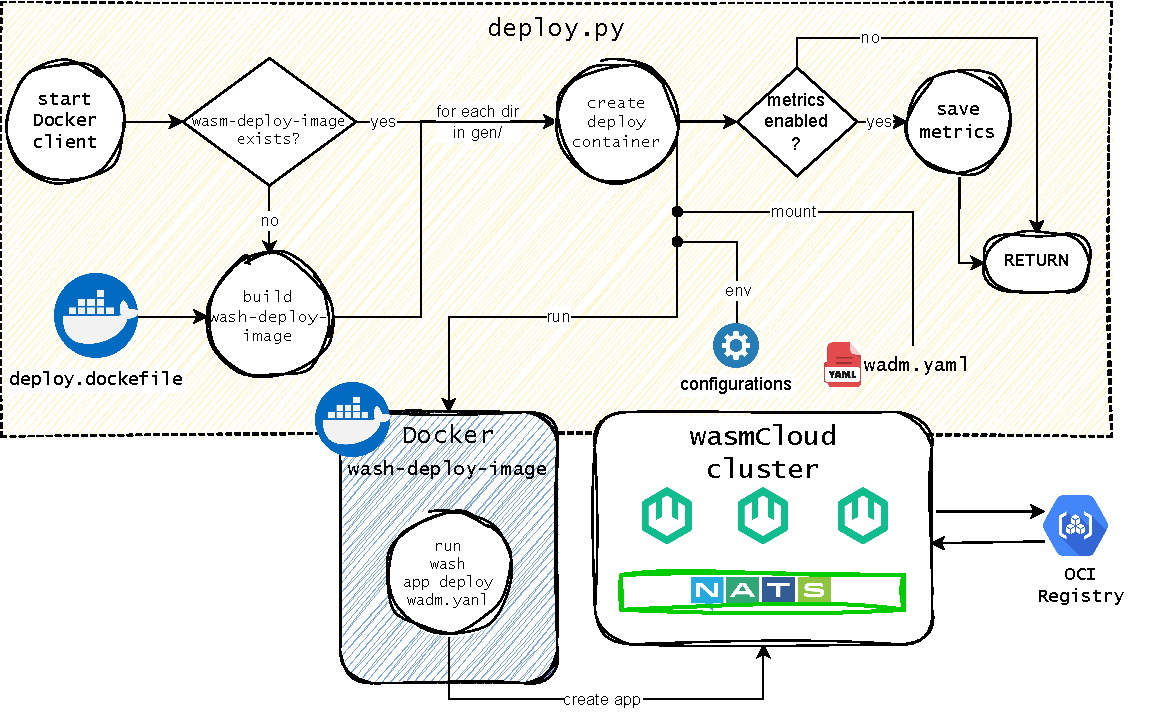
\includegraphics[width=\textwidth]{img/schemi/schemi-implementazione-deploy.drawio.pdf}
    \caption{Processo deployment applicazione su wasmCloud}
    \label{fig:impl_deploy}
\end{figure}
\FloatBarrier

\section{Utilizzo}

Adesso descriviamo la modalità di utilizzo framework, illustrandone passo dopo passo le configurazioni da impostare e le operazioni che deve eseguire l'utente. Inizieremo esplorando la struttura della repository e i file principali che la compongono, mostrati nel seguente albero.

\texttt{Pelato framework}
\dirtree{%
.1 .
.1 requirements.txt.
.1 .env.template.
.1 pelato.py.
.1 src/.
.1 infra/.
.2 wasmcloud\_edge\_host/.
.2 wasmcloud\_platform/.
.1 project/.
.1 plot\_metrics.py.
.1 benchmark/.
}

I file possono essere organizzati in categorie in base alla loro funzione:

\begin{itemize}
    \item \texttt{requirements.txt} e \texttt{.env.template} servono per configurare l'ambiente di esecuzione e il comportamento del framework
    \item il file \texttt{pelato.py} e la cartella \texttt{src/} raccolgono il codice essenziale per il funzionamento del framework
    \item la cartella \texttt{infra/} contiene degli esempi di tool e configurazioni che facilitano la creazione dell'infrastruttura su cui si appoggia wasmCloud
    \item \texttt{project/} contiene un esempio di progetto per facilitare l'utilizzo del framework da parte dell'utente
    \item \texttt{plot\_metrics.py} e \texttt{benchmark/} sono tool utilizzabili per ottenere dei grafici partendo dalle metriche 
\end{itemize}


\subsection{Configurazione framework}

\subsubsection{Virtual Environment}
Iniziamo con la configurazione del framework. Come già detto in precedenza il codice è scritto in Python, quindi sarà necessario avere un interprete di Python3 installato (consigliato \texttt{Python 3.12}), inoltre sarà necessario installare le librerie specificate nel \texttt{requirement.txt}.\\
L'approccio consigliato è quello di utilizzare un virtual environment, cioè un'istanza dell'interprete Python che consente di installare le librerie localmente, senza toccare l'interprete configurato nel sistem a o preoccuparsi di eventuali incompatibilità. Per creare il virtual environment è necessario il paccheto \texttt{venv} (installato di default per versioni successive alla 3.4). Il seguente comando

\begin{lstlisting}[language=bash]
    $ python3 -m venv .venv
\end{lstlisting}
consente di creare un environment chiamato \texttt{.venv} (di fatto una cartella nel file system). Una volta creato, l'environment deve essere attivato tramite il comando 
\begin{lstlisting}[language=bash]
    $ source .venv/bin/activate
\end{lstlisting}

A questo punto è possibile utilizzare \texttt{pip} per installare le librerie all'interno dell'environment
\begin{lstlisting}[language=bash]
    $ pip install -r requirement.txt
\end{lstlisting}

Le istruzioni riportate sono indicate per l'esecuzione all'interno di un sistema Linux.

\subsubsection{Variabili d'ambiente}

Il framework può essere configurato tramite variabili d'ambiente, ottenute dal sistema all'inizio di ogni esecuzione. Per facilitare il processo di configurazione è possibile creare un file \texttt{.env} situato nella cartella del framework: all'inizio di ogni esecuzione il file .env viene parsato e le variabili al suo interno vengono utilizzate per impostare il servizio.\\
All'interno della repositori è predisposto il file \texttt{.env.template}, nel quale sono riportate le variabili d'ambienti impostabili e la configurazione di default, che viene riportata di seguito:

\begin{lstlisting}[language=bash, caption={Variabili d'ambiente per la configurazione del framework}, captionpos=b, label={code:env}]
    REGISTRY_URL=
    REGISTRY_USER=
    REGISTRY_PASSWORD=
    PARALLEL_BUILD=True
    NATS_HOST=localhost
    NATS_PORT=4222
    ENABLE_METRICS=True
\end{lstlisting}

Andiamo ad analizzarle:
\begin{itemize}
    \item \texttt{REGISTRY\_URL}, \texttt{REGISTRY\_USER}, \texttt{REGISTRY\_PASSWORD} servono per impostare le informazioni del registry in cui verranno caricate le immagini OCI dei moduli Wasm
    \item \texttt{PARALLEL\_BUILD} abilita l'esecuzione dei container in modalità parallela
    \item \texttt{NATS\_HOST} e \texttt{NATS\_PORT} sono utilizzati in fase di deployment e rappresentano l'istanza di NATS a cui il framework si collega per deployare le applicazioni sul cluster wasmCloud
    \item \texttt{ENABLE\_METRICS} abilita la memorizzazione delle metriche ad ogni esecuzione del codice
\end{itemize}

\subsection{Task files}

Adesso ci concentreremo sulle specifiche dei file task, cioè quelli contenenti le funzioni che verranno eseguite dai moduli Wasm. Iniziamo fornendo la struttura base di ogni task file:
\begin{lstlisting}[language=Go, caption={Struttura base file task}, captionpos=b, label={code:task_file}]
    package main
    import (
    	...
    )
    ...    
    func exec_task(arg string) string{
    
    	return ... 
    }
\end{lstlisting}

I requisiti da rispettare per la definizione sono:
\begin{itemize}
    \item il file deve avere un'estensione \texttt{.go}
    \item package impostato su main
    \item funzione di interfacciamento (cioè chiamata dal main) nominata \texttt{exec\_task}
    \item la funzione di interfacciamento deve accettare una stringa e restituire una stringa
\end{itemize}

Una volta soddisfatti questi requisiti è possibile eseguire innumerevoli operazioni, come importare librerie, definire strutture e altre funzioni. La funzione interfaccia accetta e restituisce una stringa per facilitare l'integrazione con i tipi Wasm specificati in WASI.\\
Di seguito viene riportato un esempio di file task nel quale viene eseguito un parsing e poi marshaling di un Json tramite la struttura Request

\begin{lstlisting}[language=Go, caption={Task file ed integrazione con Json}, captionpos=b, label={code:task_file_json}, keepspaces=true]
    package main
    import (
        "encoding/json"
    )
    type Request struct {
        Data int
        Name string
    }
    func exec_task(arg string) string{
        // unmarshal the data
        req := Request{}
        json.Unmarshal([]byte(arg), &req)
    
        // do some operations
        ...
        
        // return the json string
        json, _ := json.Marshal(req)
        return string(json)
    }
\end{lstlisting}

\subsection{Configurazione file Workflow}

Passiamo ora alla codifica del file \texttt{workflow.yaml}, nel quale verranno effettivamente impostati i task e il loro comportamento. 

\subsubsection{Specifica file workflow}

Il file deve essere correttamente formattato in Yaml e contenere i seguenti campi:
\begin{itemize}
    \item \texttt{project\_name} -- stringa contenente il nome del progetto, può contenere spazi e viene utilizzato principalmente nella cli e nelle metriche
    \item \texttt{tasks} -- lista contenente i vari componenti Wasm
\end{itemize}

Andando nel dettaglio, ogni elemento della lista \texttt{tasks} deve contenere:
\begin{itemize}
    \item \texttt{name} --  stringa contenente il nome del componente, può contenere spazi e verrà impostato come nome dell'applicazione su wasmCloud
    \item \texttt{type} -- stringa contenente il template da utilizzare come base
    \item \texttt{code} -- stringa contenente il nome del file task da associare al componente Wasm in fase di generazione
    \item \texttt{targets} -- lista contenente delle stringhe, esse rappresentano la label \texttt{host-type} associata ai nodi target di deployment dei componenti Wasm
    \item \texttt{source\_topic} -- stringa contenente il topic da cui verranno ricevuti i dati
    \item \texttt{dest\_topic} -- stringa contenente il topic a cui verranno inviati
    \item \texttt{component\_name} -- stringa contenente il nome sintetico del componente, non può contenere spazi e funge da nome per l'OCI artifact associato
    \item \texttt{version} -- versione del componente, specificata nel formato \texttt{x.x.x}. Insieme al component\_name conferisce il nome all'OCI artifact
    
\end{itemize}

\subsubsection{Template}

I template sono dei progetti già sviluppati che forniscono certe funzionalità e fungono da base per il codice fornito dall'utente. Attualmente sono implementati due template:
\begin{itemize}
    \item \texttt{processor\_nats} -- comunicazione interamente basata su NATS: i dati arrivano da un topic e vengono inviati ad un topic
    \item \texttt{http\_producer\_nats} -- i dati possono provenire sia da un topic NATS che da una richiesta POST effettuata al nodo in cui è deployata l'applicazione. Viene utilizzato infatti l'http provider per esporre un web server nella porta 8000
\end{itemize}

Questo approccio consente una facile estendibilità del progetto: infatti potranno essere sviluppati ed aggiunti nuovi template per aumentare le funzionalità disponibili sul framework. Un altro template attualmente in sviluppo è quello per la scrittura dei dati su un DB relazionale.

\subsubsection{Esempio conversione temperatura}

Per comprendere meglio le modalità di utilizzo del file workflow analizziamo il seguente esempio:

\begin{lstlisting}[language=yaml, caption={Esempio Workflow file con processor e producer}, captionpos=b, label={code:workflow_file}, keepspaces=true]
project_name: Temperature data analysis
tasks:
  - name: Temp data conversion
    type: http_producer_nats
    code: convert.go
    targets:
      - edge
    source_topic: living_room_celsius_data
    dest_topic: living_room_kelvin_data
    component_name: celsius_to_kelvin_conversion
    version: 1.0.0
  - name: Data filter
    type: processor_nats
    code: filter.go
    targets:
      - cloud
    source_topic: living_room_kelvin_data
    dest_topic: filtered_kelvin_data
    component_name: temp_filter
    version: 1.0.2
\end{lstlisting}

In questo file workflow[\ref{code:workflow_file}] vengono definiti due componenti:
\begin{itemize}
    \item il primo si occupa di ricevere dati inviati da sensori ad un server http, convertire le temperature e pubblicarli in un topic NATS
    \item il secondo filtra i risultati, magari rimuovendo errori di misurazione o aggregandoli
\end{itemize}
Questo semplice esempio vuole mostrare come con una configurazione ridotta sia possibile generare, compilare e distribuire un'applicazione che supporta casi d'uso applicabili al mondo IoT.

\subsection{PELATO cli}

Ultimiamo questo capitolo descrivendo in modo più accurato la CLI, il componente principale con cui l'utente finale si interfaccia. Iniziamo elencando i comandi disponibili:
\begin{itemize}
    \item \texttt{gen} -- generazione del codice
    \item \texttt{build} -- build e publish moduli Wasm
    \item \texttt{deploy} -- deploy applicazioni su wasmCloud
    \item \texttt{brush} -- tutte e tre le operazioni precedenti
    \item \texttt{remove} -- rimuove le applicazioni specificate da wasmcloud
\end{itemize}

I comandi devono essere invocati tramite CLI Python ed ognuno di essi necessita come ulteriore argomento la path della cartella in cui sono contenuti il file \texttt{workflow.yaml} e le \texttt{task}, quindi degli esempi potrebbero essere:

\begin{lstlisting}[language=bash, caption={Cheatsheet comandi Pelato CLI}, captionpos=b, label={code:pelato_cli}]
    $ python3 pelato.py -h      # help, restituisce la lista dei comandi utilizzabili

    $ python3 pelato.py gen /home/lore/documents/project/   # generazione codice partendo con una path globale
    $ python3 pelato.py build ./project/    # build progetto con path locale
    $ python3 pelato.py deploy project/     # deploy applicazioni
    $ python3 pelato.py remove project/     # rimozione applicazioni 

    $ python3 pelato.py brush project/      # esecuzione pipeline gen -> build -> deploy
    
    $ python3 pelato.py test                # errore, restituisce il messaggio di help    
\end{lstlisting}
